Nek5000 solves the unsteady incompressible two-dimensional,
axisymmetric, or three-dimensional Stokes or Navier-Stokes
equations with forced or natural convection heat transfer in
both stationary (fixed) or time-dependent geometry. It also solves the compressible Navier-Stokes in the Low Mach regime, the magnetohydrodynamic equation (MHD).
The solution variables are the fluid velocity
\(\mathbf u=(u_{x},u_{y},u_{z})\), the pressure \(p\),
the temperature \(T\). 
%, mesh velocity \({\bf w}=(w_{x},w_{y},w_{z})\) (for time-dependent geometry).
%,independent passive scalar fields \(\phi_{i}\), {\footnotesize i=1,2,\ldots},
%and magnetic field \({\bf B}=(B_{x},B_{y},B_{z})\) (for MHD).
All of the above field variables
are functions of space \({\bf x}=(x,y,z)\) and time \(t\)
in domains \(\Omega_f\) and/or \(\Omega_s\) defined in Fig. \ref{fig:domains}.
Additionally Nek5000 can handle conjugate heat transfer problems.

\begin{figure}
\centering
%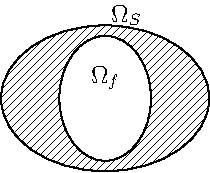
\includegraphics[width=0.3\textwidth]{domains}
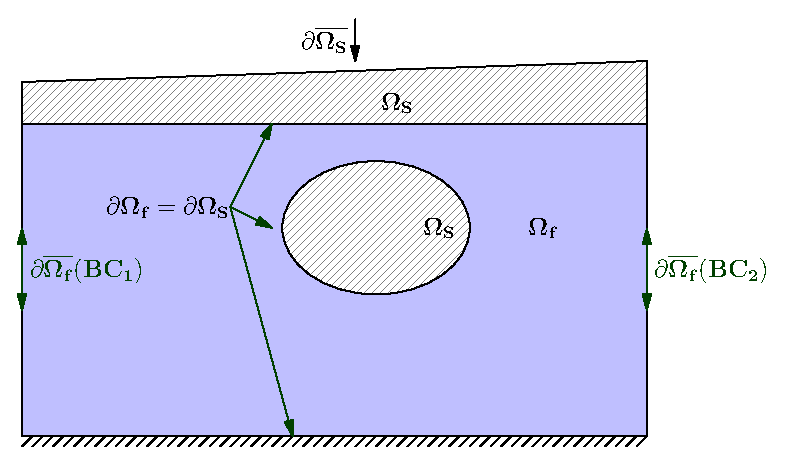
\includegraphics[width=0.8\textwidth]{walls}
\caption{Computational domain showing respective fluid
and solid subdomains, \(\Omega_f\) and \(\Omega_s\). The shared boundaries are denoted \(\partial\Omega_f=\partial\Omega_s\) and the solid boundary which is not shared by fluid is \(\overline{\partial\Omega_s}\), while the fluid boundary not shared by solid \(\overline{\partial\Omega_f}\).}
\label{fig:domains}
\end{figure}

\section{Incompressible Navier--Stokes equations}
%
The governing equations of flow motion in dimensional form are
\begin{eqnarray}\label{eq:ns_momentum}
\rho(\partial_{t} \mathbf u +\mathbf u \cdot \nabla \mathbf u) = - \nabla p + \nabla \cdot \tau + \rho {\bf f} \,\, , \text{in } \Omega_f , \quad \text{  (Momentum)  } 
\end{eqnarray}
where \( \tau=\mu[\nabla \vect u+\nabla \vect u^{T}]\).
\begin{eqnarray}\label{eq:ns_cont}
 \nabla \cdot \mathbf u =0 \,\, , \text{in } \Omega_f, \quad \text{  (Continuity)  }   
\end{eqnarray}

If the fluid viscosity is constant in the entire domain the viscous stress tensor can be contracted \(\nabla\cdot\tau=\mu\Delta \vect u\), therefore one may solve the Navier--Stokes equations in either the stress formulation, or no stress

\begin{itemize}
\item Variable viscosity requires the full stress tensor \(\nabla \cdot \tau=\nabla \cdot \mu[\nabla \vect u+\nabla \vect u^{T}]\), and we shall refer to this as the stress formulation
\item Constant viscosity leads to a simpler stress tensor \(\nabla \cdot \tau=\mu\Delta \vect u\), which we refer to as the 'no stress' formulation
\end{itemize}

\section{Non-dimensional Navier-Stokes}
Let us introduce the following non-dimensional variables \(\vect x^*\ = \frac{\vect x}{L}\), \(\vect u^*\ = \frac{u}{U}\), \(t^*\ = \frac{t}{L/U}\,\).
For the pressure scale we have two options 
\begin{itemize}
\item convective effects are dominant i.e. high velocity flows
\( p^* = \frac{p}{\rho U^2} \)
\item viscous effects are dominant i.e. creeping flows (Stokes flow)
\( p^* = \frac{p L}{\mu U} \)
\end{itemize}
For highly convective flows we choose the first scaling of the pressure and obtain the non-dimensional Navier-Stokes:
\begin{equation}\label{eq:NS_nondim}
\frac{\partial \mathbf{u^*}}{\partial t^*} + \mathbf{u^*} \cdot \nabla \mathbf{u^*}\ = -\nabla p^* + \frac{1}{Re} \nabla\cdot \tau^* + \frac{1}{Fr}\frac{\mathbf{f}}{g}.
\end{equation}
where \( \tau^*=[\nabla \vect u^*+\nabla \vect u^{*T}]\).
The two non-dimensional numbers here are the Reynolds number \(Re=\frac{\nu}{U L}\) \(Fr\) and the Froude number, defined as \(Fr = \frac{U^2}{gL}\).
%The above governing equations are subject to boundary conditions
%and initial conditions described in the following sections.
%
%\begin{tabular}{ l|l|l|l| }
%   \hline
%   Equation &  & &\\ \hline \hline
%   Incompressible NS (stress)& \ref{eq:ns_momentum} & \ref{eq:ns_cont}, \((4)=0\) & \\ 
%   Incompressible NS (non-stress)& \ref{eq:ns_momentum}, \((3)=\Delta \vect u\) & \ref{eq:ns_cont}, \((4)=0\) \\ 
%   Incompressible NS (non-stress)+Energy& \ref{eq:ns_momentum}, \((3)=\Delta \vect u\) & \ref{eq:ns_cont},\((4)=0\)& \ref{eq:energy} \\ 
%   Unsteady Stokes (non-stress)& \ref{eq:ns_momentum}, \((2)=0\( & \ref{eq:ns_cont},\((4)=0\)&  \\ 
%   Steady Stokes (non-stress)& \ref{eq:ns_momentum}, \((1)=0\), \((2)=0\) & \ref{eq:ns_cont},\((4)=0\)&  \\
%   Steady Heat transfer& --- & ---&  \ref{eq:energy}, \((5)=0\), \((6)=0\)\\
%   Compressible NS, Low Mach (non-stress)& \ref{eq:ns_momentum}, \((3)=\Delta \vect u\) & \ref{eq:ns_cont}, \((4)\neq 0\) \ref{eq:energy} + EOS &\ref{eq:energy} \\ 
%   \hline
%\end{tabular}

%\newline
\section{Energy equation}
In addition to the fluid flow, Nek5000 computes automatically the energy equation
\begin{eqnarray}\label{eq:energy}
 \rho c_{p} ( \partial_{t} T + \mathbf u \cdot \nabla T ) =
   \nabla \cdot (k \nabla T) + q_{vol}\,\, ,\text{in } \Omega_f\cup \Omega_s  \text{  (Energy)  } 
\end{eqnarray}

\section{Non-dimensional energy/passive scalar equation}
A similar non-dimensionalization as for the flow equations using the non-dimensional variables
\(\vect x^*\ = \frac{\vect x}{L}\),  \(\vect u^*\ = \frac{u}{U}\), \(t^*\ = \frac{t}{L/U}\), \(T=\frac{T^*-T_0}{\delta T}\) leads to
\begin{eqnarray}\label{eq:energy_nondim}
\partial_{t^*} T^* + \vect u^* \cdot \nabla T^* =
  \frac{1}{Pe} \nabla \cdot \nabla T^* + q_{vol}\,\, ,\text{in } \Omega_f\cup \Omega_s  \text{  (Energy)  } 
\end{eqnarray}
where \(Pe=LU/\alpha\), with \(\alpha=k/\rho c_p\).


\section{Passive scalars}\label{sec:passive_scal}

We can additionally solve a convection-diffusion equation for each passive scalar \(\phi_i\),
\(i\)=1,2,\(\ldots\) in \(\Omega_f \cup \Omega_s\)
\begin{eqnarray}\label{eq:pass_scal}
   (\rho c_{p})_i ( \partial_{t} \phi_{i} + \mathbf u \cdot \nabla \phi_{i} ) =
   \nabla \cdot (k_i \nabla \phi_{i}) + (q_{vol})_i.
\end{eqnarray}

The terminology and
restrictions of the temperature equations are retained for
the passive scalars, so that it is the responsibility of the
user to convert the notation of the passive scalar
parameters to their thermal analogues.
For example, in the context of mass transfer,
the user should recognize that the values specified
for temperature and heat flux
will represent concentration and mass flux, respectively.
Any combination of these equation characteristics is permissible with the
following restrictions. First, the equation must be set to unsteady if it is
time-dependent or if there is any type of advection. For these cases, the
steady-state (if it exists) is found as stable evolution of the
initial-value-problem. Secondly, the stress formulation must be selected if
the geometry is time-dependent. In addition, stress formulation must be
employed if there are traction boundary conditions applied on any fluid
boundary, or if any mixed velocity/traction boundaries, such as symmetry and
outflow/n, are not aligned with either one of the Cartesian \(x,y\) or \(z\) axes.
Other capabilities of Nek5000 are the linearized Navier-Stokes for flow stability, magnetohydrodynamic flows etc.



\section{Unsteady Stokes }
In the case of flows dominated by viscous effects Nek5000 can solve the reduced Stokes equations
\begin{eqnarray}\label{eq:ns_momentum_stokes}
 \rho(\partial_{t} \mathbf u ) = - \nabla p + \nabla \cdot \tau + \rho {\bf f} \,\, , \text{in } \Omega_f \text{  (Momentum)  }
\end{eqnarray}
where \(\nabla \cdot\tau=\nabla\cdot\mu[\nabla \vect u+\nabla \vect u^{T}]\) and
\begin{eqnarray}\label{eq:ns_cont_stokes}
 \nabla \cdot \mathbf u =0 \,\, , \text{in } \Omega_f  \text{  (Continuity)  } 
\end{eqnarray}
Also here we can distinguish between the stress and non-stress formulation according to whether the viscosity is variable or not. The non-dimensional form of these equations can be obtained using the viscous scaling of the pressure.


\section{Steady Stokes }
If there is no time-dependence, then Nek5000 can further reduce to
\begin{eqnarray}\label{eq:ns_momentum_steady_stokes}
 - \nabla p + \nabla \cdot \tau + \rho {\bf f}=0 \,\, , \text{in } \Omega_f \text{  (Momentum)  }
\end{eqnarray}
where \(\nabla \cdot\tau=\nabla\cdot\mu[\nabla \vect u+\nabla {\vect u}^{T}]\) and
\begin{eqnarray}\label{eq:ns_cont_steady_stokes}
 \nabla \cdot \mathbf u =0 \,\, , \text{in } \Omega_f  \text{  (Continuity)  } 
\end{eqnarray}

\section{Linearized Equations}
In addition to the basic evolution equations described above, Nek5000
provides support for the evolution of small perturbations about
a base state by solving the {\em linearized equations}
\begin{equation} \label{eq:pertu}
  \rho(\partial_{t} {\mathbf u_i}' + \mathbf u \cdot \nabla {\mathbf u_i}^{'} + \mathbf u_i' \cdot \nabla \mathbf u) =
   - \nabla p_i' + \mu \nabla^2 \mathbf u_i', \qquad \nabla \cdot \mathbf u_i' = 0,
\end{equation}
for multiple perturbation fields \(i=1,2,\dots\) subject to different initial
conditions and (typically) homogeneous boundary conditions.  
These solutions can be evolved concurrently with the base fields \((\mathbf u,p,T)\).
There is also
support for computing perturbation solutions to the Boussinesq equations for
natural convection.  Calculations such as these can be used to estimate Lyapunov exponents of chaotic flows, etc.



\section{Steady conduction}    
The energy Eq.~\ref{eq:energy} in which the advection term \(\mathbf u \cdot \nabla T\)
    and the transient term \(\partial_{t} T\) are zero. In essence this represents a Poisson equation.
    

\section{Low-Mach Navier-Stokes}\label{sec:lowma}
The compressible Navier-Stokes differ mathematically from the incompressible ones mainly in the divergence constraint \(\nabla \cdot \vect u\neq 0\). In this case the system of equations is not closed and an additional equation of state (EOS) is required to connect the state variables, e.g. \(p=f(\rho,T)\). However Nek5000 can only solve the Low Mach approximation of the compressible Navier-Stokes. The Low-Mach approximation decouples the pressure from the velocity leading to a system of equations which can be solved numerically in a similar fashion as the incompressible Navier-Stokes.

The Low Mach equations in non-dimensional form are 
\begin{eqnarray}
&&\rho\bigg(\frac{\d \vect u}{\d t}+ \vect u\cdot\nabla\vect u\bigg)=-\nabla p+\nabla \cdot\bb\tau+\rho\vect f\ \\ \nonumber
&&\frac{\d \vect \rho}{\d t}+ \vect u\cdot\nabla\vect \rho=-\rho\nabla \cdot \vect u\\ \nonumber
&&\rho\bigg(\frac{\d T}{\d t}+ \vect u\cdot\nabla T\bigg)=-\nabla \cdot k \nabla T\\ \nonumber
\end{eqnarray}
where \(\bb\tau=\mu[\nabla \vect u+\nabla \vect u^{T}-\frac{2}{3}\nabla \cdot \vect u \vect I]\).


The implementation of the equation if state for the Low Mach formulation is for the moment hard-coded to be the ideal gas equation of state \(p=\rho R T\). This allows for both variable density and variable viscosity. The system is solved by substituting \(\rho=f(p,T)\) into the continuity equation and obtaining a so-called thermal divergence (the term \(\nabla \cdot \mathbf u\) is given as a function of the temperature).
A more detailed description on how these equations connect is given in section \ref{sec:lowma} as well as in the developer's manual.

\section{Incompressible MHD equations}\label{sec:mhd}
Magnetohydrodynamics is based on the idea that magnetic fields can induce currents in a moving conductive fluid, which in turn creates forces on the fluid and changing the magnetic field itself. The set of equations which describe MHD are a combination of the Navier-Stokes equations of fluid dynamics and Maxwell's equations of electromagnetism. These differential equations have to be solved simultaneously, and Nek5000 has an implementation for the incompressible MHD.

Consider a fluid of velocity \(\vect u\) subject to a magnetic field \(\vect B\) then the incompressible MHD equations are
\begin{eqnarray}
 \rho(\partial_{t} \mathbf u + \mathbf u \cdot \nabla \mathbf u) &=& - \nabla p + \mu \Delta \mathbf u + \bB\cdot \nabla \bB \ ,\\ 
 \nabla \cdot \mathbf u & =& 0\\ \nonumber
   \partial_{t} \bB + \mathbf u \cdot \nabla \bB &=& - \nabla q + \eta \Delta \bB + \bB\cdot \nabla \mathbf u \ ,\\ 
    \nabla \cdot \bB & =& 0 \nonumber
\end{eqnarray}
where \(\rho\) is the density \(\mu\) the viscosity, \(\eta\) resistivity, and pressure \(p\).


The total magnetic field can be split into two parts: \( \mathbf{B} = \mathbf{B_0} + \mathbf{b} \) (mean + fluctuations). The above equations become in terms of Els\"asser variables (\(\mathbf{z}^{\pm} =  \mathbf{u} \pm \mathbf{b} \)) 
\begin{eqnarray}
\frac{\partial {\mathbf{z}^{\pm}}}{\partial t}\mp\left(\mathbf {B}_0\cdot{\mathbf \nabla}\right){\mathbf z^{\pm}} + \left({\mathbf z^{\mp}}\cdot{\mathbf \nabla}\right){\mathbf z^{\pm}} = -{\mathbf \nabla}p 
+ \nu_+ \nabla^2 \mathbf{z}^{\pm} + \nu_- \nabla^2 \mathbf{z}^{\mp} 
\end{eqnarray}
where \( \nu_\pm = \nu \pm \eta \).

The important non-dimensional parameters for MHD are \(Re = U L /\nu \) and the magnetic Re \( Re_M = U L /\eta \).
